\documentclass[letterpaper,10pt]{book}
% Change to 10 pt
\usepackage{pdfpages}
\usepackage{morewrites}			% to counteract the no write space problem
\setcounter{tocdepth}{6}

\usepackage[framemethod=TikZ]{mdframed}

\usepackage{fancyhdr}

\usepackage{paralist}
\usepackage{amsmath}
\usepackage{amsfonts}
\usepackage{amssymb}
\usepackage{graphicx}

\usepackage{datetime}
%\usepackage{ulem}

%\usepackage[nottoc]{toobibind}

\usepackage[inline]{enumitem}

% Outer margin at 2.50 is exacty correct to fit the ``corruption alert'' tables
\usepackage[inner=1.0in, outer=2.50in, top=2.54cm,bottom=2.54cm, marginparwidth=2.25in]{geometry}

\usepackage{marginnote}
\usepackage{longtable}
\usepackage{booktabs}
\usepackage{xcolor}

\usepackage{soul}

%%%%%%%%%%%%
\definecolor{ForestGreen}{rgb}{0.00,0.29,0.098}
%%%%%%%%%%%%

\usepackage{marginnote}

\usepackage{imakeidx} 
\usepackage[
	backref=true,
	style=numeric,
%	citestyle=numeric,
	backend=bibtex
	]{biblatex}
\usepackage[driverfallback=hypertex,colorlinks=True]{hyperref}
\usepackage{cleveref}

\makeindex[name=scripture,columnsep=20pt, columnseprule=True,columns=3, title=Scripture References]
\makeindex[name=speaker,columnsep=20pt, columnseprule=True,,columns=2, title=Sermon Creator]
\makeindex[name=series,columnsep=20pt, columnseprule=True,,columns=2, title=Sermon Series]
\makeindex[name=date,columnsep=20pt, columnseprule=True,columns=2, title=Sermon Date]
\makeindex[name=event,columnsep=20pt, columnseprule=True,columns=2, title=Event]
\makeindex[name=topic,columnsep=20pt, columnseprule=True,columns=2, title=Topic]
\makeindex[name=AWIP,columnsep=20pt, columnseprule=True,columns=3, title=All Words in Passage]
\makeindex[name=NWIV,columnsep=20pt, columnseprule=True,columns=3, title=Number of Words in Verse]
\makeindex[name=PNIP,columnsep=20pt, columnseprule=True,columns=3, title=Proper Names in Passage]
\makeindex[name=PEIP,columnsep=20pt, columnseprule=True,columns=2, title=Prophetic Events in Passage]
\makeindex[name=TWPAQ,columnsep=20pt, columnseprule=True,columns=1, title=13-Word Phrases and Quotes]
\makeindex[name=PFTTIS,columnsep=20pt, columnseprule=False,columns=3, title=Phrases found 13 times in scripture]
\makeindex[name=WFTTIS,columnsep=20pt, columnseprule=False,columns=3, title=Words found 13 times in scripture]
\makeindex[name=WFITV,columnsep=20pt, columnseprule=False,columns=3, title=Words found in exactly 13 verses]
\makeindex[name=EVENTS,columnsep=20pt, columnseprule=False,columns=2, title=Sermon Log by Place]
\makeindex[name=QUESTIONS,columnsep=20pt, columnseprule=False,columns=2, title=Bible Questions]
\makeindex[name=DOCTRINES,columnsep=20pt, columnseprule=False,columns=2, title=Doctrines]
\makeindex[name=SONGS,columnsep=20pt, columnseprule=False,columns=1, title=Songs]
\makeindex[name=LOCATION,columnsep=20pt, columnseprule=False,columns= 2, title=Location]
\makeindex[name=FACEBOOK,columnsep=20pt, columnseprule=False,columns=2, title=Facebook]
\makeindex[name=DEVOTIONAL,columnsep=20pt, columnseprule=False,columns=2, title=Devotional Items]
%%%%%%%%%%%%%%%%% EXTRA COLORS
\definecolor{champagne}{rgb}{0.97,0.91,0.81}
\definecolor{bone}{rgb}{0.89,0.85,0.79}
\pagestyle{fancy}
\fancyhf{}
\fancyhead[LE,RO]{\today}
\fancyhead[RE,LO]{Daily Bible Reading}
\fancyhead[CE,CO]{-page \thepage  - }

\fancyfoot[CO,CE]{\leftmark}
%\fancyfoot[LE,RO]{CSCE 692, HW1}

\title{DBR\\
Daily \\ Reads}
\author{Keith Anthony \\
\today }
%+/ffffff +   \pagenumbering{gobble}
\bibliography{Bibliographies/All20220122}

\setlength{\fboxsep}{1.0pt}

\usepackage[utf8]{inputenc}
\usepackage{tikz}

\begin{document}
%%%%%%%%%%%% Tile Page

\begin{titlepage}

\begin{flushright}
\rightskip=-2.5cm
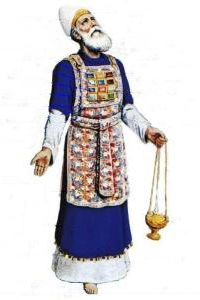
\includegraphics[width=50mm,scale=1.5]{Extras/Melchisedec.jpg}
\vspace{0.4in}  % Create a title for the document and write it in bold font
\LARGE{\textbf{\date}} % Again, do a line break
\linebreak 
% Create a subtitle \large{with Outlines, Statistics, Cross References, and Notes}
\vspace{0.5in}
\begin{flushleft}
\LARGE{Day \#72: Sunday, 13 March 2022 PLAIN  \\}\vspace{0.25in}
\LARGE{Joshua 22-24 Psalm 72 Proverb 13}
\end{flushleft}
\vspace{0.6in}
\bigskip

\normalsize{Xenia, Oh.\\}
\normalsize{created: \today}
\vspace{1.3in}

\end{flushright}
\end{titlepage}

\newpage 
\tableofcontents\hypertarget{TOC}{}
\listoffigures
\listoftables

\hyphenation{A-bim-e-lech bre-thren E-phra-im  Gib-e-o-nites Jer-u-sa-lem through-out Phil-i-stines The-o-phil-us Am-a-le-kites ven-geance Mesh-el-e-mi-ah onan-ism Phar-a-oh thoughts grev-ous-ness Hach-a-liah adul-ter-er Shad-rach}

%%%%%%%%%%%%%%%%% EXTRA COLORS
%%%%%%%%%%%%%%%%% EXTRA COLORS
%%%%%%%%%%%%%%%%% EXTRA COLORS
\definecolor{champagne}{rgb}{0.97,0.91,0.81}
\definecolor{bone}{rgb}{0.89,0.85,0.79}

\definecolor{ForestGreen}{rgb}{0.00,0.29,0.098}
\definecolor{GIVING}{cmyk}{1,0.0,0.72,.1}

\definecolor{MLPE}{cmyk}{1,1,0,.45}
\definecolor{SOCCER}{cmyk}{.77, 0, .42, .49}
\definecolor{PAYBILL}{cmyk}{0,0.83,0.76,0.07}
\definecolor{SERMON}{cmyk}{.14,.9,0,.30} % aka seance \href{http://www.flatuicolorpicker.com/purple-cmyk-color-model/}{seance}
\definecolor{BIBLE}{cmyk}{0,.17,.74,.17}
\definecolor{WORKBLUE}{cmyk}{1, .5, 0, .6}
\definecolor{myOrange}{cmyk}{0, .4, .98, .03}
\definecolor{myTan}{cmyk}{0.0,.07,.17,.10}
\definecolor{myRed}{cmyk}{0,1,1,0}
\definecolor{myWhite}{cmyk}{0,0,0,0}
\definecolor{BLUESoD}{cmyk}{.97,.84,0,.04}
\definecolor{WHITE}{cmyk}{0,0,0,0}
\definecolor{OLDGOLD}{cmyk}{0.05,0.3,1.00,0}
\definecolor{CASTLETON}{cmyk}{1,0,0.31,0.66}
\definecolor{cadmiumgreen}{rgb}{0.0, 0.42, 0.24}
\definecolor{jungle}{rgb}{0.203,0.4882,0.1718}
\definecolor{MYGOLD}{rgb}{1,.84,0}

\definecolor{MYLIGHTGRAY}{rgb}{.85,.85,.85}

\definecolor{codegreen}{rgb}{0,0.6,0}
\definecolor{codegray}{rgb}{0.5,0.5,0.5}
\definecolor{codepurple}{rgb}{0.58,0,0.82}
\definecolor{backcolour}{rgb}{0.95,0.95,0.92}


\mdfdefinestyle{MyFrame}{%
    linecolor=blue,
    outerlinewidth=2pt,
    roundcorner=5pt,
    innertopmargin=\baselineskip,
    innerbottommargin=\baselineskip,
    innerrightmargin=10pt,
    innerleftmargin=10pt,
    backgroundcolor=gray!25!white}


\mdfdefinestyle{MyFrame2}{%
    linecolor=black,
    outerlinewidth=2pt,
    roundcorner=5pt,
    innertopmargin=\baselineskip,
    innerbottommargin=\baselineskip,
    innerrightmargin=10pt,
    innerleftmargin=10pt,
    backgroundcolor=yellow!25!white}


%%%%%
%% for PFTTIS list
%%%%%

%%% And Joseph said unto
\index[PFTTIS]{And Joseph said unto!Genesis!Gen 40:008}
\index[PFTTIS]{And Joseph said unto!Genesis!Gen 40:012}
\index[PFTTIS]{And Joseph said unto!Genesis!Gen 41:025}
\index[PFTTIS]{And Joseph said unto!Genesis!Gen 42:014}
\index[PFTTIS]{And Joseph said unto!Genesis!Gen 42:018}
\index[PFTTIS]{And Joseph said unto!Genesis!Gen 44:015}
\index[PFTTIS]{And Joseph said unto!Genesis!Gen 45:003}
\index[PFTTIS]{And Joseph said unto!Genesis!Gen 45:004}
\index[PFTTIS]{And Joseph said unto!Genesis!Gen 46:031}
\index[PFTTIS]{And Joseph said unto!Genesis!Gen 48:009}
\index[PFTTIS]{And Joseph said unto!Genesis!Gen 48:018}
\index[PFTTIS]{And Joseph said unto!Genesis!Gen 50:019}
\index[PFTTIS]{And Joseph said unto!Genesis!Gen 50:024}


%%% a shadow
\index[PFTTIS]{a shadow!1Chronicles!1Chr 029:15}
\index[PFTTIS]{a shadow!Job!Job 008:09}
\index[PFTTIS]{a shadow!Job!Job 014:02}
\index[PFTTIS]{a shadow!Job!Job 017:07}
\index[PFTTIS]{a shadow!Psalm!Psa 102:011}
\index[PFTTIS]{a shadow!Psalm!Psa 144:004}
\index[PFTTIS]{a shadow!Ecclesiastes!Eccl 006:012}
\index[PFTTIS]{a shadow!Ecclesiastes!Eccl 008:013}
\index[PFTTIS]{a shadow!Isaiah!Isa 04:006}
\index[PFTTIS]{a shadow!Isaiah!Isa 25:004}
\index[PFTTIS]{a shadow!Jonah!Jnh 04:06}
\index[PFTTIS]{a shadow!Colossians!Col 02:017}
\index[PFTTIS]{a shadow!Hebews!Heb 10:001}

%%% blessed is the man
\index[PFTTIS]{blessed is the man!Psalm!Psa 001:001}
\index[PFTTIS]{blessed is the man!Psalm!Psa 032:002}
\index[PFTTIS]{blessed is the man!Psalm!Psa 034:008}
\index[PFTTIS]{blessed is the man!Psalm!Psa 065:004}
\index[PFTTIS]{blessed is the man!Psalm!Psa 084:005}
\index[PFTTIS]{blessed is the man!Psalm!Psa 084:012}
\index[PFTTIS]{blessed is the man!Psalm!Psa 094:012}
\index[PFTTIS]{blessed is the man!Psalm!Psa 112:001}
\index[PFTTIS]{blessed is the man!Proverbs!Pro 008:034}
\index[PFTTIS]{blessed is the man!Isaiah!Isa 056:002}
\index[PFTTIS]{blessed is the man!Jeremiah!Jer 017:007}
\index[PFTTIS]{blessed is the man!Romans!Rom 004:008}
\index[PFTTIS]{blessed is the man!James!Jam 001:012}


%%% carry them
\index[PFTTIS]{carry them!Leviticus!Lev 14:045}
\index[PFTTIS]{carry them!Numbers!Num 11:012}
\index[PFTTIS]{carry them!Joshua!Jsh 04:003}
\index[PFTTIS]{carry them!1Samuel!1Sam 20:040}
\index[PFTTIS]{carry them!1Kings!1Kng 08:046}
\index[PFTTIS]{carry them!2Chronicles!2Chr 06:036}
\index[PFTTIS]{carry them!Ezra!Ezra 05:015}
\index[PFTTIS]{carry them!Isaiah!Isa 40:011}
\index[PFTTIS]{carry them!Isaiah!Isa 41:016}
\index[PFTTIS]{carry them!Isaiah!Isa 57:013}
\index[PFTTIS]{carry them!Jeremiah!Jer 20:004}
\index[PFTTIS]{carry them!Jeremiah!Jer 20:005}
\index[PFTTIS]{carry them!Jeremiah!Jer 43:012}


\index[PFTTIS]{good tidings!2Samuel!2Sam 18:027}
\index[PFTTIS]{good tidings!1Kings!1Ki 01:042}
\index[PFTTIS]{good tidings!2Kings!2Ki 07:009 (2x)}
\index[PFTTIS]{good tidings!Isaiah!Isa 40:009 (2x)}
\index[PFTTIS]{good tidings!Isaiah!Isa 41:007}
\index[PFTTIS]{good tidings!Isaiah!Isa 52:007}
\index[PFTTIS]{good tidings!Isaiah!Isa 61:001}
\index[PFTTIS]{good tidings!Nahum!Nah 01:005}
\index[PFTTIS]{good tidings!Luke!Lk 02:010}
\index[PFTTIS]{good tidings!1Thessalonians!1Thess 03:006}


%%% dead body
\index[PFTTIS]{dead body!Leviticus!Lev 21:011}
\index[PFTTIS]{dead body!Numbers!Num 06:006}
\index[PFTTIS]{dead body!Numbers!Num 09:006}
\index[PFTTIS]{dead body!Numbers!Num 09:007}
\index[PFTTIS]{dead body!Numbers!Num 09:010}
\index[PFTTIS]{dead body!Numbers!Num 09:011}
\index[PFTTIS]{dead body!Numbers!Num 09:013}
\index[PFTTIS]{dead body!Numbers!Num 09:016}
\index[PFTTIS]{dead body!2Kings!2Ki 08:005}
\index[PFTTIS]{dead body!Isaiah!Isa 26:019}
\index[PFTTIS]{dead body!Jeremiah!Jer 26:023}
\index[PFTTIS]{dead body!Jeremiah!Jer 36:030}
\index[PFTTIS]{dead body!Haggai!Hag 02:013}

%%% great sea
\index[PFTTIS]{great sea!Numbers!Num 34:006}
\index[PFTTIS]{great sea!Numbers!Num 34:007}
\index[PFTTIS]{great sea!Joshua!Jos 01:004}
\index[PFTTIS]{great sea!Joshua!Jos 09:001}
\index[PFTTIS]{great sea!Joshua!Jos 15:012}
\index[PFTTIS]{great sea!Joshua!Jos 15:047}
\index[PFTTIS]{great sea!Joshua!Jos 23:004}
\index[PFTTIS]{great sea!Ezekiel!Eze 47:010}
\index[PFTTIS]{great sea!Ezekiel!Eze 47:015}
\index[PFTTIS]{great sea!Ezekiel!Eze 47:019}
\index[PFTTIS]{great sea!Ezekiel!Eze 47:020}
\index[PFTTIS]{great sea!Ezekiel!Eze 48:028}
\index[PFTTIS]{great sea!Daniel!Dan 07:002}


%%% have forsaken me
\index[PFTTIS]{have forsaken me!Judges!Jdg 10:013}
\index[PFTTIS]{have forsaken me!1Samuel!1Sam 08:008}
\index[PFTTIS]{have forsaken me!1Kings!1Ki 11:033}
\index[PFTTIS]{have forsaken me!2Kings!2Ki 22:017}
\index[PFTTIS]{have forsaken me!2Chronicles!2Chr 12:005}
\index[PFTTIS]{have forsaken me!2Chronicles!2Chr 34:025}
\index[PFTTIS]{have forsaken me!Jeremiah!Jer 01:016}
\index[PFTTIS]{have forsaken me!Jeremiah!Jer 02:013}
\index[PFTTIS]{have forsaken me!Jeremiah!Jer 05:007}
\index[PFTTIS]{have forsaken me!Jeremiah!Jer 05:019}
\index[PFTTIS]{have forsaken me!Jeremiah!Jer 16:011 (2x)}
\index[PFTTIS]{have forsaken me!Jeremiah!Jer 19:004}

%%% no king
\index[PFTTIS]{no king!Judges!Jdg 17:06}
\index[PFTTIS]{no king!Judges!Jdg 18:01}
\index[PFTTIS]{no king!Judges!Jdg 19:01}
\index[PFTTIS]{no king!Judges!Jdg 21:25}
\index[PFTTIS]{no king!1Kings!1Ki 22:47}
\index[PFTTIS]{no king!2Kings!2Ki 23:25}
\index[PFTTIS]{no king!Nehemiah!Neh 13:26}
\index[PFTTIS]{no king!Psalms!Psa 033:016}
\index[PFTTIS]{no king!Proverbs!Pro 30:27}
\index[PFTTIS]{no king!Daniel!Dan 02:10}
\index[PFTTIS]{no king!Hosea!Hos 10:03}
\index[PFTTIS]{no king!Micah!Mic 04:09}
\index[PFTTIS]{no king!John!Jhn 19:15}


%%% rebellious house
\index[PFTTIS]{rebellious house!Exodus!Exo 02:005}
\index[PFTTIS]{rebellious house!Exodus!Exo 02:006}
\index[PFTTIS]{rebellious house!Exodus!Exo 02:008}
\index[PFTTIS]{rebellious house!Exodus!Exo 03:009}
\index[PFTTIS]{rebellious house!Exodus!Exo 03:026}
\index[PFTTIS]{rebellious house!Exodus!Exo 03:027}
\index[PFTTIS]{rebellious house!Exodus!Exo 12:002 (2x)}
\index[PFTTIS]{rebellious house!Exodus!Exo 12:003}
\index[PFTTIS]{rebellious house!Exodus!Exo 12:009}
\index[PFTTIS]{rebellious house!Exodus!Exo 12:025}
\index[PFTTIS]{rebellious house!Exodus!Exo 17:012}
\index[PFTTIS]{rebellious house!Exodus!Exo 24:003}

%%% seek him
\index[PFTTIS]{seek him!Deuteronomy!Deu 04:029}\index[PFTTIS]{seek him!1Samuel!1Sam 23:025}
\index[PFTTIS]{seek him!1Chronicles!1Chr 28:009}
\index[PFTTIS]{seek him!2Chronicles!1Chr 15:002}
\index[PFTTIS]{seek him!Ezra!Ezr 08:022}
\index[PFTTIS]{seek him!Psalms!Psa 022:026}
\index[PFTTIS]{seek him!Psalms!Psa 024:006}
\index[PFTTIS]{seek him!Psalms!Psa 119:002}
\index[PFTTIS]{seek him!SoS!SoS 03:002}
\index[PFTTIS]{seek him!SoS!SoS 06:001}
\index[PFTTIS]{seek him!Hosea!Hos 07:010}
\index[PFTTIS]{seek him!Amos!Amo 05:008}
\index[PFTTIS]{seek him!Hebrews!Heb 11:0063}


%%% seek ye
\index[PFTTIS]{seek ye!Isaiah!Isa 34:016}
\index[PFTTIS]{seek ye!Isaiah!Isa 45:019}
\index[PFTTIS]{seek ye!Isaiah!Isa 55:006}
\index[PFTTIS]{seek ye!Amos!Amos 5:004}
\index[PFTTIS]{seek ye!John!John 1:38}
\index[PFTTIS]{seek ye!John!John 18:4}
\index[PFTTIS]{seek ye!John!John 18:7}
\index[PFTTIS]{seek ye!Matthew!Matt 6:33}
\index[PFTTIS]{seek ye!Numbers!Num 16:10}
\index[PFTTIS]{seek ye!Luke!Luke 12:31}
\index[PFTTIS]{seek ye!Luke!Luke 24:5}
\index[PFTTIS]{seek ye!Psalm!Psa 27:8}
\index[PFTTIS]{seek ye!Zephaniah!Zeph 2:3}

%%% the uncircumcised
\index[PFTTIS]{the uncircumcised!Genesis!Gen 17:014}
\index[PFTTIS]{the uncircumcised!Judges!Jdg 14:003}
\index[PFTTIS]{the uncircumcised!Judges!Jdg 15:018}
\index[PFTTIS]{the uncircumcised!2Samuel!2Sam 01:020}
\index[PFTTIS]{the uncircumcised!Isaiah!Isa 02:001}
\index[PFTTIS]{the uncircumcised!Jeremiah!Jer 09:025}
\index[PFTTIS]{the uncircumcised!Ezekiel!Eze 28:010}
\index[PFTTIS]{the uncircumcised!Ezekiel!Eze 31:018}
\index[PFTTIS]{the uncircumcised!Ezekiel!Eze 32:019}
\index[PFTTIS]{the uncircumcised!Ezekiel!Eze 32:027}
\index[PFTTIS]{the uncircumcised!Ezekiel!Eze 32:028}
\index[PFTTIS]{the uncircumcised!Ezekiel!Eze 32:029}
\index[PFTTIS]{the uncircumcised!Ezekiel!Eze 32:032}

%%% worship him
\index[PFTTIS]{worship him!Psalms!Psa 97:007}
\index[PFTTIS]{worship him!Zephaniah!Zeph 02:011}
\index[PFTTIS]{worship him!Matthew!Matt 02:002}
\index[PFTTIS]{worship him!Matthew!Matt 02:008}
\index[PFTTIS]{worship him!John!John 04:023}
\index[PFTTIS]{worship him!John!John 04:024 (2x)} 
\index[PFTTIS]{worship him!Acts!Acts 17:023}
\index[PFTTIS]{worship him!Hebrews!Heb 01:006}
\index[PFTTIS]{worship him!Revelation!Rev 04:010}
\index[PFTTIS]{worship him!Revelation!Rev 13:008}
\index[PFTTIS]{worship him!Revelation!Rev 14:007}
\index[PFTTIS]{worship him!Revelation!Rev 19:010}


%%%%%
%% for PFTTIS list
%%%%%

%%% afflictions
\index[WFTTIS]{afflictions!Psalms!Psa 34:019}
\index[WFTTIS]{afflictions!Psalms!Psa 132:001}
\index[WFTTIS]{afflictions!Acts!Acts 07:010}
\index[WFTTIS]{afflictions!Acts!Acts 20:023}
\index[WFTTIS]{afflictions!2Corinthians!2Cor 06:004}
\index[WFTTIS]{afflictions!Colossians!Col 01:024}
\index[WFTTIS]{afflictions!1Thessalonians!1Thess 03:003}
\index[WFTTIS]{afflictions!2Timothy!2Tim 01:008}
\index[WFTTIS]{afflictions!2Timothy!2Tim 03:011}
\index[WFTTIS]{afflictions!2Timothy!2Tim 04:005}
\index[WFTTIS]{afflictions!Hebrews!Heb 10:032}
\index[WFTTIS]{afflictions!Hebrews!Heb 10:033}
\index[WFTTIS]{afflictions!1Peter!1Pet 05:009}

%%% acsend
\index[WFTTIS]{acsend!Joshua!Jos 06:05}
\index[WFTTIS]{acsend!Psalm!Psa 024:003}
\index[WFTTIS]{acsend!Psalm!Psa 135:007}
\index[WFTTIS]{acsend!Psalm!Psa 139:008}
\index[WFTTIS]{acsend!Isaiah!Isa 14:013}
\index[WFTTIS]{acsend!Isaiah!Isa 14:014}
\index[WFTTIS]{acsend!Jeremiah!Jer 10:013}
\index[WFTTIS]{acsend!Jeremiah!Jer 51:016}
\index[WFTTIS]{acsend!Ezekiel!Eze 38:009}
\index[WFTTIS]{acsend!John!John 06:062}
\index[WFTTIS]{acsend!John!John 20:017}
\index[WFTTIS]{acsend!Romans!Rom 10:006}
\index[WFTTIS]{acsend!Revelation!Rev 17:008}

%%% Assyrian
\index[WFTTIS]{Assyrian!Isaiah!Isa 10:005}
\index[WFTTIS]{Assyrian!Isaiah!Isa 10:024}
\index[WFTTIS]{Assyrian!Isaiah!Isa 14:025}
\index[WFTTIS]{Assyrian!Isaiah!Isa 19:023}
\index[WFTTIS]{Assyrian!Isaiah!Isa 23:013}
\index[WFTTIS]{Assyrian!Isaiah!Isa 30:031}
\index[WFTTIS]{Assyrian!Isaiah!Isa 31:008}
\index[WFTTIS]{Assyrian!Isaiah!Isa 52:004}
\index[WFTTIS]{Assyrian!Ezekiel!Eze 31:003}
\index[WFTTIS]{Assyrian!Hosea!Hos 05:013}
\index[WFTTIS]{Assyrian!Hosea!Hos 11:005}
\index[WFTTIS]{Assyrian!Micah!Hos 05:005}
\index[WFTTIS]{Assyrian!Micah!Hos 05:006}

%%% blot
\index[WFTTIS]{blot!Exodus!Exo 32:032}
\index[WFTTIS]{blot!Exodus!Exo 32:033}
\index[WFTTIS]{blot!Numbers!Num 05:026}
\index[WFTTIS]{blot!Deuteronomy!Deut 09:014}
\index[WFTTIS]{blot!Deuteronomy!Deut 25:019}
\index[WFTTIS]{blot!Deuteronomy!Deut 29:020}
\index[WFTTIS]{blot!2Kings!2Ki 14:027}
\index[WFTTIS]{blot!Job!Job 31:007}
\index[WFTTIS]{blot!Psalms!Psa 51:001}
\index[WFTTIS]{blot!Psalms!Psa 51:009}
\index[WFTTIS]{blot!Proverbs!Pro 09:007}
\index[WFTTIS]{blot!Jeremiah!Jer 18:023}
\index[WFTTIS]{blot!Revelation!Rev 03:005}


%%% chain
\index[WFTTIS]{chain!Genesis!Gen 41:042}
\index[WFTTIS]{chain!1Kings!1Ki 07:017}
\index[WFTTIS]{chain!Psalms!Psa 73:006}
\index[WFTTIS]{chain!SoS!Sos 04:009}
\index[WFTTIS]{chain!Lamentations!Lam 03:007}
\index[WFTTIS]{chain!Ezekiel!Eze 07:023}
\index[WFTTIS]{chain!Ezekiel!Eze 16:011}
\index[WFTTIS]{chain!Daniel!Dan 05:007}
\index[WFTTIS]{chain!Daniel!Dan 05:016}
\index[WFTTIS]{chain!Daniel!Dan 05:029}
\index[WFTTIS]{chain!Acts!Acts 28:020}
\index[WFTTIS]{chain!2Timothy!2Tim 01:016}
\index[WFTTIS]{chain!Revelation!Rev 20:001}


%%% controversy
\index[WFTTIS]{controversy!Deuteronomy!Deu 17:008}
\index[WFTTIS]{controversy!Deuteronomy!Deu 19:017}
\index[WFTTIS]{controversy!Deuteronomy!Deu 21:005}
\index[WFTTIS]{controversy!Deuteronomy!Deu 25:001}
\index[WFTTIS]{controversy!2Samuel!2Sam 15:002}
\index[WFTTIS]{controversy!Isaiah!Isa 34:008}
\index[WFTTIS]{controversy!Jeremiah!Jer 25:031}
\index[WFTTIS]{controversy!Ezekiel!Eze 44:024}
\index[WFTTIS]{controversy!Hosea!Hos 04:001}
\index[WFTTIS]{controversy!Hosea!Hos 12:002}
\index[WFTTIS]{controversy!Micah!Mic 06:002 (2x)}
\index[WFTTIS]{controversy!1Timothy!1Tim 03:016}


%%% Dagon/Dagon's
\index[WFTTIS]{Dagon!Judges!Jdg 16:023}
\index[WFTTIS]{Dagon!1Samuel!1Sam 05:002 (2x)}
\index[WFTTIS]{Dagon!1Samuel!1Sam 05:003 (2x)}
\index[WFTTIS]{Dagon!1Samuel!1Sam 05:004 (3x)}
\index[WFTTIS]{Dagon!1Samuel!1Sam 05:005 (3x)}
\index[WFTTIS]{Dagon!1Samuel!1Sam 05:007}
\index[WFTTIS]{Dagon!1Chronicles!1Chr 10:010}

%%% disobedient
\index[WFTTIS]{disobedient!1Kings!1Ki 13:026}
\index[WFTTIS]{disobedient!Nehemiah!Neh 09:026}
\index[WFTTIS]{disobedient!Luke!Luke 01:017}
\index[WFTTIS]{disobedient!Acts!Acts 26:019}
\index[WFTTIS]{disobedient!Romans!Rom 01:030}
\index[WFTTIS]{disobedient!Romans!Rom 10:021}
\index[WFTTIS]{disobedient!1Timothy!1Tim 01:009}
\index[WFTTIS]{disobedient!2Timothy!2Tim 03:002}
\index[WFTTIS]{disobedient!Titus!Titus 01:016}
\index[WFTTIS]{disobedient!Titus!Titus 03:003}
\index[WFTTIS]{disobedient!1Peter!1Pet 02:007}
\index[WFTTIS]{disobedient!1Peter!1Pet 02:008}
\index[WFTTIS]{disobedient!1Peter!1Pet 03:020}


%%% doubt
\index[WFTTIS]{doubt!Genesis!Gen 37:033}
\index[WFTTIS]{doubt!Deuteronomy!Deu 28:066}
\index[WFTTIS]{doubt!Job!Job 12:002}
\index[WFTTIS]{doubt!Matthew!Matt 14:031}
\index[WFTTIS]{doubt!Matthew!Matt 21:021}
\index[WFTTIS]{doubt!Mark!Mk 11:023}
\index[WFTTIS]{doubt!Luke!Lk 11:020}
\index[WFTTIS]{doubt!John!Jhn 10:024}
\index[WFTTIS]{doubt!Acts!Acts 02:012}
\index[WFTTIS]{doubt!Acts!Acts 28:004}
\index[WFTTIS]{doubt!1Corinthians!1Cor 09:010}
\index[WFTTIS]{doubt!Galatians!Gal 04:020}
\index[WFTTIS]{doubt!1John!1Jhn 02:019}


%%% dungeon
\index[WFTTIS]{dungeon!Genesis!Gen 40:015}
\index[WFTTIS]{dungeon!Genesis!Gen 41:014}
\index[WFTTIS]{dungeon!Exodus!Exo 12:029}
\index[WFTTIS]{dungeon!Jeremiah!Jer 37:016}
\index[WFTTIS]{dungeon!Jeremiah!Jer 38:006 (2x)}
\index[WFTTIS]{dungeon!Jeremiah!Jer 38:007}
\index[WFTTIS]{dungeon!Jeremiah!Jer 38:009}
\index[WFTTIS]{dungeon!Jeremiah!Jer 38:010}
\index[WFTTIS]{dungeon!Jeremiah!Jer 38:011}
\index[WFTTIS]{dungeon!Jeremiah!Jer 38:013}
\index[WFTTIS]{dungeon!Lamentations!Lam 03:053}
\index[WFTTIS]{dungeon!Lamentations!Lam 03:055}


%%% error
\index[WFTTIS]{error!2Samuel!2Sam 06:007}
\index[WFTTIS]{error!Job!Job 19:004}
\index[WFTTIS]{error!Ecclesiastes!Ecc 05:006}
\index[WFTTIS]{error!Ecclesiastes!Ecc 10:005}
\index[WFTTIS]{error!Isaiah!Isa 32:006}
\index[WFTTIS]{error!Daniel!Dan 06:004}
\index[WFTTIS]{error!Matthew!Matt 27:064}
\index[WFTTIS]{error!Romans!Rom 01:027}
\index[WFTTIS]{error!James!Jam 05:020}
\index[WFTTIS]{error!2Peter!2Pet 02:018}
\index[WFTTIS]{error!2Peter!2Pet 03:017}
\index[WFTTIS]{error!1John!1Jn 04:006}
\index[WFTTIS]{error!Jude!Jude 01:011}

%%% fourish
\index[WFTTIS]{fourish!Psalms!Psa 072:007}
\index[WFTTIS]{fourish!Psalms!Psa 072:016}
\index[WFTTIS]{fourish!Psalms!Psa 092:007}
\index[WFTTIS]{fourish!Psalms!Psa 092:012}
\index[WFTTIS]{fourish!Psalms!Psa 092:013}
\index[WFTTIS]{fourish!Psalms!Psa 132:018}
\index[WFTTIS]{fourish!Proverbs!Pro 11:28}
\index[WFTTIS]{fourish!Proverbs!Pro 14:11}
\index[WFTTIS]{fourish!Ecclesiastes!Ecc 12:05}
\index[WFTTIS]{fourish!SongOfSolomon!SOS 07:12}
\index[WFTTIS]{fourish!Isaiah!Isa 17:11}
\index[WFTTIS]{fourish!Isaiah!Isa 66:14}
\index[WFTTIS]{fourish!Ezekiel!Eze 17:24}




%%% giants
\index[WFTTIS]{giants!Genesis!Gen 06:004}
\index[WFTTIS]{giants!Numbers!Num 13:033}
\index[WFTTIS]{giants!Deuteronomy!Deut 02:011}
\index[WFTTIS]{giants!Deuteronomy!Deut 02:021}
\index[WFTTIS]{giants!Deuteronomy!Deut 03:011}
\index[WFTTIS]{giants!Deuteronomy!Deut 03:013}
\index[WFTTIS]{giants!Joshua!Josh 12:004}
\index[WFTTIS]{giants!Joshua!Josh 13:012}
\index[WFTTIS]{giants!Joshua!Josh 15:008}
\index[WFTTIS]{giants!Joshua!Josh 17:015}
\index[WFTTIS]{giants!Joshua!Josh 16:016}

%%% good man
\index[WFTTIS]{good man!2 Samuel!2Sa 18:27}
%(1) Psalms 37:23 [5]
%(1) Psalms 112:5 [2]
%(1) Proverbs 12:2 [2]
%(1) Proverbs 13:22 [2]
%(1) Proverbs 14:14 [14]
%(1) Micah 7:2 [2]
%(1) Matthew 12:35 [2]
%(1) Luke 6:45 [2]
%(1) Luke 23:50 [15]
%(1) John 7:12 [17]
%(1) Acts 11:24 [5]
%(1) Romans 5:7 [14]

%%% Hinnom
\index[WFTTIS]{Hinnom!Joshua!Jsh 15:008}
\index[WFTTIS]{Hinnom!Joshua!Jsh 18:016}
\index[WFTTIS]{Hinnom!2Kings!2Ki 23:010}
\index[WFTTIS]{Hinnom!2Chronicles!2Chr 28:003}
\index[WFTTIS]{Hinnom!2Chronicles!2Chr 33:006}
\index[WFTTIS]{Hinnom!Nehemiah!Neh 11:030}
\index[WFTTIS]{Hinnom!Jeremiah!Jer 07:031}
\index[WFTTIS]{Hinnom!Jeremiah!Jer 07:032}
\index[WFTTIS]{Hinnom!Jeremiah!Jer 19:002}
\index[WFTTIS]{Hinnom!Jeremiah!Jer 19:006}
\index[WFTTIS]{Hinnom!Jeremiah!Jer 32:035}

%%% inclined
\index[WFTTIS]{inclined!Judges!Jdg 09:003}
\index[WFTTIS]{inclined!Psalms!Psa 040:001}
\index[WFTTIS]{inclined!Psalms!Psa 116:002}
\index[WFTTIS]{inclined!Psalms!Psa 119:112}
\index[WFTTIS]{inclined!Proverbs!Pro 05:13}
\index[WFTTIS]{inclined!Jeremiah!Jer 07:24}
\index[WFTTIS]{inclined!Jeremiah!Jer 07:26}
\index[WFTTIS]{inclined!Jeremiah!Jer 11:08}
\index[WFTTIS]{inclined!Jeremiah!Jer 17:23}
\index[WFTTIS]{inclined!Jeremiah!Jer 25:04}
\index[WFTTIS]{inclined!Jeremiah!Jer 34:14}
\index[WFTTIS]{inclined!Jeremiah!Jer 35:15}
\index[WFTTIS]{inclined!Jeremiah!Jer 44:05}


%%% laughed
\index[WFTTIS]{laughed!Genesis!Gen 17:017}
\index[WFTTIS]{laughed!Genesis!Gen 18:012}
\index[WFTTIS]{laughed!Genesis!Gen 18:015}
\index[WFTTIS]{laughed!2Kings!2Ki 19:021}
\index[WFTTIS]{laughed!2Chronicles!2Chr 30:010}
\index[WFTTIS]{laughed!Nehemiah!Neh 02:019}
\index[WFTTIS]{laughed!Job!Job 12:004}
\index[WFTTIS]{laughed!Job!Job 29:024}
\index[WFTTIS]{laughed!Isaiah!Isa 37:022}
\index[WFTTIS]{laughed!Ezekiel!Ezek 23:032}
\index[WFTTIS]{laughed!Matthew!Matt 09:024}
\index[WFTTIS]{laughed!Mark!Mk 05:040}
\index[WFTTIS]{laughed!Luke!Lk 08:053}

%%% liar
\index[WFTTIS]{liar!Job!Job 24:025}
\index[WFTTIS]{liar!Proverbs!Pro 17:004}
\index[WFTTIS]{liar!Proverbs!Pro 19:022}
\index[WFTTIS]{liar!Proverbs!Pro 30:006}
\index[WFTTIS]{liar!Jeremiah!Jer 15:018}
\index[WFTTIS]{liar!John!Jhn 08:044}
\index[WFTTIS]{liar!John!Jhn 08:055}
\index[WFTTIS]{liar!Romans!Rom 03:004}
\index[WFTTIS]{liar!1John!1Jhn 01:010}
\index[WFTTIS]{liar!1John!1Jhn 02:004}
\index[WFTTIS]{liar!1John!1Jhn 02:022}
\index[WFTTIS]{liar!1John!1Jhn 04:020}
\index[WFTTIS]{liar!1John!1Jhn 05:010}

%%% palsy
\index[WFTTIS]{palsy!Matthew!Matt 04:024}
\index[WFTTIS]{palsy!Matthew!Matt 08:006}
\index[WFTTIS]{palsy!Matthew!Matt 09:002}
\index[WFTTIS]{palsy!Matthew!Matt 09:006}
\index[WFTTIS]{palsy!Mark!Mk 02:003}
\index[WFTTIS]{palsy!Mark!Mk 02:004}
\index[WFTTIS]{palsy!Mark!Mk 02:005}
\index[WFTTIS]{palsy!Mark!Mk 02:009}
\index[WFTTIS]{palsy!Mark!Mk 02:010}
\index[WFTTIS]{palsy!Luke!Lk 05:018}
\index[WFTTIS]{palsy!Luke!Lk 05:024}
\index[WFTTIS]{palsy!Acts!Acts 09:033}

%%% Profitable
\index[WFTTIS]{profitable!Job!Job 22:002 (2x)}
\index[WFTTIS]{profitable!Ecclesiastes!Ecc 10:010}
\index[WFTTIS]{profitable!Isaiah!Isa 44:010}
\index[WFTTIS]{profitable!Jeremiah!Jer 13:007}
\index[WFTTIS]{profitable!Matthew!Matt 05:029}
\index[WFTTIS]{profitable!Matthew!Matt 05:030}
\index[WFTTIS]{profitable!Acts!Acts 20:020}
\index[WFTTIS]{profitable!1Timothy!1Tim 04:008}
\index[WFTTIS]{profitable!2Timothy!2Tim 03:016}
\index[WFTTIS]{profitable!2Timothy!2Tim 04:011}
\index[WFTTIS]{profitable!Titus!Titus 03:008}
\index[WFTTIS]{profitable!Philemon!Phlm 01:011}

%%% Rechab
\index[WFTTIS]{Rechab!2Samuel!2Sam 04:002}
\index[WFTTIS]{Rechab!2Samuel!2Sam 04:005}
\index[WFTTIS]{Rechab!2Samuel!2Sam 04:006}
\index[WFTTIS]{Rechab!2Samuel!2Sam 04:009}
\index[WFTTIS]{Rechab!2KIngs!2Ki 10:015}
\index[WFTTIS]{Rechab!2KIngs!2Ki 10:023}
\index[WFTTIS]{Rechab!1Chronicles!1Chr 02:055}
\index[WFTTIS]{Rechab!Nehemiah!Neh 03:014}
\index[WFTTIS]{Rechab!Jeremiah!Jer 35:006}
\index[WFTTIS]{Rechab!Jeremiah!Jer 35:008}
\index[WFTTIS]{Rechab!Jeremiah!Jer 35:014}
\index[WFTTIS]{Rechab!Jeremiah!Jer 35:016}
\index[WFTTIS]{Rechab!Jeremiah!Jer 35:019}

%%% serpents
\index[WFTTIS]{serpents!Exodus!Exo 07:012}
\index[WFTTIS]{serpents!Numbers!Num 21:006}
\index[WFTTIS]{serpents!Numbers!Num 21:007}
\index[WFTTIS]{serpents!Deuteronomy!Deu 08:015}
\index[WFTTIS]{serpents!Deuteronomy!Deu 32:024}
\index[WFTTIS]{serpents!Jeremiah!Jer 08:017}
\index[WFTTIS]{serpents!Matthew!Matt 10:016}
\index[WFTTIS]{serpents!Matthew!Matt 23:033}
\index[WFTTIS]{serpents!Mark!Mk 16:018}
\index[WFTTIS]{serpents!Luke!Lk 10:019}
\index[WFTTIS]{serpents!1Corinthians!1Cor 10:009}
\index[WFTTIS]{serpents!James!Jas 03:007}
\index[WFTTIS]{serpents!Revelation!Rev 09:019}

%%% short
\index[WFTTIS]{short!Numbers!Num 11:023}
\index[WFTTIS]{short!2Kings!2Ki 10:032}
\index[WFTTIS]{short!Job!Job 17:012}
\index[WFTTIS]{short!Job!Job 20:005}
\index[WFTTIS]{short!Psalms!Psa 89:047}
\index[WFTTIS]{short!Romans!Rom 03:023}
\index[WFTTIS]{short!Romans!Rom 09:028  (2x)}
\index[WFTTIS]{short!1Corinthians!1Cor 07:029}
\index[WFTTIS]{short!1Thessalonians!1Thess 02:017}
\index[WFTTIS]{short!Hebrews!Heb 04:001}
\index[WFTTIS]{short!Revelation!Rev 12:012}
\index[WFTTIS]{short!Revelation!Rev 17:010}

%%% smiteth
\index[WFTTIS]{smiteth!Exodus!Exo 21:012}
\index[WFTTIS]{smiteth!Exodus!Exo 21:15}
\index[WFTTIS]{smiteth!Deuteronomy!Dt 25:11}
\index[WFTTIS]{smiteth!Deuteronomy!Dt 27:24}
\index[WFTTIS]{smiteth!Joshua!Jsh 15:16}
\index[WFTTIS]{smiteth!Judges!Jdg 15:16}
\index[WFTTIS]{smiteth!2 Samuel!2Sa 05:08}
\index[WFTTIS]{smiteth!1Chronicles!1Chr 11:06}
\index[WFTTIS]{smiteth!Job!1Chr 26:12}
\index[WFTTIS]{smiteth!Isaiah!Isa 09:13}
\index[WFTTIS]{smiteth!Lamentations!Lam 03:30}
\index[WFTTIS]{smiteth!Ezekiel!Eze 07:09}
\index[WFTTIS]{smiteth!Luke!Lk 06:29}



%%% vanities
\index[WFTTIS]{vanities!Deuteronomy!Deut 21:021}
\index[WFTTIS]{vanities!1Kings!1Ki 16:013}
\index[WFTTIS]{vanities!1Kings!1Ki 16:026}
\index[WFTTIS]{vanities!Psalms!Psa 031:006}
\index[WFTTIS]{vanities!Ecclesiastes!Ecc 01:002 (2x)}
\index[WFTTIS]{vanities!Ecclesiastes!Ecc 05:007}
\index[WFTTIS]{vanities!Ecclesiastes!Ecc 12:008}
\index[WFTTIS]{vanities!Jeremiah!Jer 08:019}
\index[WFTTIS]{vanities!Jeremiah!Jer 10:008}
\index[WFTTIS]{vanities!Jeremiah!Jer 14:022}
\index[WFTTIS]{vanities!Jonah!Jnh 02:008}
\index[WFTTIS]{vanities!Acts!Acts 14:015}



%%%%%
%% for PFTTIS list
%%%%%

%%% worm
\index[WFITV]{worm!Exodus!Exo 16:024}
\index[WFITV]{worm!Job!Job 17:014}
\index[WFITV]{worm!Job!Job 24:029}
\index[WFITV]{worm!Job!Job 25:005 (2x)}
\index[WFITV]{worm!Psalms!Psa 022:006}
\index[WFITV]{worm!Isaiah!Isa 14:011}
\index[WFITV]{worm!Isaiah!Isa 41:014}
\index[WFITV]{worm!Isaiah!Isa 51:008}
\index[WFITV]{worm!Isaiah!Isa 66:024}
\index[WFITV]{worm!Jonah!Jnh 04:007}
\index[WFITV]{worm!Mark!Mk 09:044}
\index[WFITV]{worm!Mark!Mk 09:046}
\index[WFITV]{worm!Mark!Mk 09:048}


%\subsubsection{Title}
%\textbf{Introduction:} Isaiah 46 
%\index[speaker]{Speaker!Isaiah 49 (Title}
%\index[series]{Book (Speaker)!IPassage (Title)}
%\index[date]{2017/07/09!Isaiah 49 (Title)}
%\begin{compactenum}[I.]
%    \item  \textbf{Point} \index[scripture]{Isaiah!IPassage} (IPassage)
%\end{compactenum}




  

\chapter{Joshua 22}

% \textcolor[cmyk]{0.99998,1,0,0}{
\marginpar{\scriptsize \centering \fcolorbox{bone}{lime}{\textbf{BACK TO THE OTHER SIDE}}\\ (Joshua 22)

\begin{compactenum}[I.][8]

    \item The \textbf{Two-and-a-Half} \index[scripture]{Joshua!Jsh 22:01}(Jsh 22:1)
    \item \textbf{Toward the East} \index[scripture]{Joshua!Jsh 22:05}(Jsh 22:5)
    \item \textbf{Trouble at Church} \index[scripture]{Joshua!Jsh 22:11}(Jsh 22:11)
    \item \textbf{Tension} \index[scripture]{Joshua!Jsh 22:12}(Jsh 22:12)
    \item A \textbf{Testimony to Unity} \index[scripture]{Joshua!Jsh 22:27}(Jsh 22:27)

\end{compactenum}}

\footnote{\textcolor[rgb]{0.00,0.25,0.00}{\hyperlink{TOC}{Return to end of Table of Contents.}}}\footnote{\href{https://audiobible.com/bible/joshua_22.html}{\textcolor[cmyk]{0.99998,1,0,0}{Joshua 22 Audio}}}\textcolor[cmyk]{0.99998,1,0,0}{Then Joshua called the Reubenites, and the Gadites, and the half tribe of Manasseh,}
[2] \textcolor[cmyk]{0.99998,1,0,0}{And said unto them, Ye have kept all that Moses the servant \fcolorbox{bone}{bone}{of the LORD} commanded you, and have obeyed my voice in all that I commanded you:}
[3] \textcolor[cmyk]{0.99998,1,0,0}{Ye have not left your brethren these many days unto this day, but have kept the charge of the commandment \fcolorbox{bone}{bone}{of the LORD} your God.}
[4] \textcolor[cmyk]{0.99998,1,0,0}{And now the LORD your God hath given rest unto your brethren, as he promised them: therefore now return ye, and get you unto your tents, \emph{and} unto the land of your possession, which Moses the servant \fcolorbox{bone}{bone}{of the LORD} gave you on the other side Jordan.}
[5] \textcolor[cmyk]{0.99998,1,0,0}{But take diligent heed to do the commandment and the law, which Moses the servant \fcolorbox{bone}{bone}{of the LORD} charged you, to love the LORD your God, and to walk in all his ways, and to keep his commandments, and to cleave unto him, and to serve him with all your heart and with all your soul.}
[6] \textcolor[cmyk]{0.99998,1,0,0}{So Joshua blessed them, and sent them away: and they went unto their tents.}\\
\\
\P \textcolor[cmyk]{0.99998,1,0,0}{Now to the \emph{one} half of the tribe of Manasseh Moses had given \emph{possession} in Bashan: but unto the \emph{other} half thereof gave Joshua among their brethren on this side Jordan westward. And when Joshua sent them away also unto their tents, then he blessed them,}
[8] \textcolor[cmyk]{0.99998,1,0,0}{And he spake unto them, saying, Return with much riches unto your tents, and with very much cattle, with silver, and with gold, and with brass, and with iron, and with very much raiment: divide the spoil of your enemies with your brethren.}\\
\\
\P \textcolor[cmyk]{0.99998,1,0,0}{And the children of Reuben and the children of Gad and the half tribe of Manasseh returned, and departed from the children of Israel out of Shiloh, which \emph{is} in the land of Canaan, to go unto the country of Gilead, to the land of their possession, whereof they were possessed, according to the word \fcolorbox{bone}{bone}{of the LORD} by the hand of Moses.}\\
\\
\P \textcolor[cmyk]{0.99998,1,0,0}{And when they came unto the borders of Jordan, that \emph{are} in the land of Canaan, the children of Reuben and the children of Gad and the half tribe of Manasseh built there an altar by Jordan, a great altar to see to.}\\
\\
\P \textcolor[cmyk]{0.99998,1,0,0}{And the children of Israel heard say, Behold, the children of Reuben and the children of Gad and the half tribe of Manasseh have built an altar over against the land of Canaan, in the borders of Jordan, at the passage of the children of Israel.}
[12] \textcolor[cmyk]{0.99998,1,0,0}{And when the children of Israel heard \emph{of} \emph{it}, the whole congregation of the children of Israel gathered themselves together at Shiloh, to go up to war against them.}
[13] \textcolor[cmyk]{0.99998,1,0,0}{And the children of Israel sent unto the children of Reuben, and to the children of Gad, and to the half tribe of Manasseh, into the land of Gilead, Phinehas the son of Eleazar the priest,}
[14] \textcolor[cmyk]{0.99998,1,0,0}{And with him ten princes, of each chief house a prince throughout all the tribes of Israel; and each one \emph{was} an head of the house of their fathers among the thousands of Israel.}\\
\\
\P \textcolor[cmyk]{0.99998,1,0,0}{And they came unto the children of Reuben, and to the children of Gad, and to the half tribe of Manasseh, unto the land of Gilead, and they spake with them, saying,}
[16] \textcolor[cmyk]{0.99998,1,0,0}{Thus saith the whole congregation \fcolorbox{bone}{bone}{of the LORD}, What trespass \emph{is} this that ye have committed against the God of Israel, to turn away this day from following the LORD, in that ye have builded you an altar, that ye might rebel this day against the LORD?}
[17] \textcolor[cmyk]{0.99998,1,0,0}{\emph{Is} the iniquity of Peor too little for us, from which we are not cleansed until this day, although there was a plague in the congregation \fcolorbox{bone}{bone}{of the LORD},}
[18] \textcolor[cmyk]{0.99998,1,0,0}{But that ye must turn away this day from following the LORD? and it will be, \emph{seeing} ye rebel to day against the LORD, that to morrow he will be wroth with the whole congregation of Israel.}
[19] \textcolor[cmyk]{0.99998,1,0,0}{Notwithstanding, if the land of your possession \emph{be} unclean, \emph{then} pass ye over unto the land of the possession \fcolorbox{bone}{bone}{of the LORD}, wherein the LORD'S tabernacle dwelleth, and take possession among us: but rebel not against the LORD, nor rebel against us, in building you an altar beside the altar \fcolorbox{bone}{bone}{of the LORD} our God.}
[20] \textcolor[cmyk]{0.99998,1,0,0}{Did not Achan the son of Zerah commit a trespass in the accursed thing, and wrath fell on all the congregation of Israel? and that man perished not alone in his iniquity.}\\
\\
\P \textcolor[cmyk]{0.99998,1,0,0}{Then the children of Reuben and the children of Gad and the half tribe of Manasseh answered, and said unto the heads of the thousands of Israel,}
[22] \textcolor[cmyk]{0.99998,1,0,0}{The LORD God of gods, the LORD God of gods, he knoweth, and Israel he shall know; if \emph{it} \emph{be} in rebellion, or if in \fcolorbox{bone}{MYGOLD}{transgression} against the LORD, (save us not this day,)}
[23] \textcolor[cmyk]{0.99998,1,0,0}{That we have built us an altar to turn from following the LORD, or if to offer thereon burnt offering or meat offering, or if to offer peace offerings thereon, let the LORD himself require \emph{it};}
[24] \textcolor[cmyk]{0.99998,1,0,0}{And if we have not \emph{rather} done it for fear of \emph{this} thing, saying, In time to come your children might speak unto our children, saying, What have ye to do with the LORD God of Israel?}
[25] \textcolor[cmyk]{0.99998,1,0,0}{For the LORD hath made Jordan a border between us and you, ye children of Reuben and children of Gad; ye have no part in the LORD: so shall your children make our children cease from fearing the LORD.}
[26] \textcolor[cmyk]{0.99998,1,0,0}{Therefore we said, Let us now prepare to build us an altar, not for burnt offering, nor for sacrifice:}
[27] \textcolor[cmyk]{0.99998,1,0,0}{But \emph{that} it \emph{may} \emph{be} a witness between us, and you, and our generations after us, that we might do the service \fcolorbox{bone}{bone}{of the LORD} before him with our burnt offerings, and with our sacrifices, and with our peace offerings; that your children may not say to our children in time to come, Ye have no part in the LORD.}
[28] \textcolor[cmyk]{0.99998,1,0,0}{Therefore said we, that it shall be, when they should \emph{so} say to us or to our generations in time to come, that we may say \emph{again}, Behold the pattern of the altar \fcolorbox{bone}{bone}{of the LORD}, which our fathers made, not for burnt offerings, nor for sacrifices; but it \emph{is} a witness between us and you.}
[29] \textcolor[cmyk]{0.99998,1,0,0}{God forbid that we should rebel against the LORD, and turn this day from following the LORD, to build an altar for burnt offerings, for meat offerings, or for sacrifices, beside the altar \fcolorbox{bone}{bone}{of the LORD} our God that \emph{is} before his tabernacle.}\\
\\
\P \textcolor[cmyk]{0.99998,1,0,0}{And when Phinehas the priest, and the princes of the congregation and heads of the thousands of Israel which \emph{were} with him, heard the words that the children of Reuben and the children of Gad and the children of Manasseh spake, it pleased them.}
[31] \textcolor[cmyk]{0.99998,1,0,0}{And Phinehas the son of Eleazar the priest said unto the children of Reuben, and to the children of Gad, and to the children of Manasseh, This day we perceive that the LORD \emph{is} among us, because ye have not committed this trespass against the LORD: now ye have delivered the children of Israel out of the hand \fcolorbox{bone}{bone}{of the LORD}.}\\
\\
\P \textcolor[cmyk]{0.99998,1,0,0}{And Phinehas the son of Eleazar the priest, and the princes, returned from the children of Reuben, and from the children of Gad, out of the land of Gilead, unto the land of Canaan, to the children of Israel, and brought them word again.}
[33] \textcolor[cmyk]{0.99998,1,0,0}{And the thing pleased the children of Israel; and the children of Israel blessed God, and did not intend to go up against them in battle, to destroy the land wherein the children of Reuben and Gad dwelt.}
[34] \textcolor[cmyk]{0.99998,1,0,0}{And the children of Reuben and the children of Gad called the altar \emph{Ed}: for it \emph{shall} \emph{be} a witness between us that the LORD \emph{is} God.}
\chapter{Joshua 23}

% \textcolor[cmyk]{0.99998,1,0,0}{
\marginpar{\scriptsize \centering \fcolorbox{blue}{lime}{\textbf{JOSHUA BEGINS HIS GOODBYE}}\\ (Joshua 23)

\begin{compactenum}[I.][8]

    \item \textbf{Joshua's War} \index[scripture]{Joshua!Jsh 23:03}(Jsh 23:3)
    \item \textbf{Joshua's Work} \index[scripture]{Joshua!Jsh 23:04}(Jsh 23:4)
    \item \textbf{Joshua's Warning} \index[scripture]{Joshua!Jsh 23:13}(Jsh 23:13)
    \item \textbf{Joshua's Way} \index[scripture]{Joshua!Jsh 23:14}(Jsh 23:14)
    \item \textbf{Joshua's Words} \index[scripture]{Joshua!Jsh 23:02--16}(Jsh 23:2--16)
    \item \textbf{Joshua's Witness} \index[scripture]{Joshua!Jsh 23:16}(Jsh 23:16)

\end{compactenum}}






\footnote{\textcolor[rgb]{0.00,0.25,0.00}{\hyperlink{TOC}{Return to end of Table of Contents.}}}\footnote{\href{https://audiobible.com/bible/joshua_23.html}{\textcolor[cmyk]{0.99998,1,0,0}{Joshua 23 Audio}}}\textcolor[cmyk]{0.99998,1,0,0}{And it came to pass a long time after that the LORD had given rest unto Israel from \fcolorbox{bone}{bone}{all} their enemies round about, that Joshua waxed old \emph{and} stricken in age.}
[2] \textcolor[cmyk]{0.99998,1,0,0}{And Joshua called for \fcolorbox{bone}{bone}{all} Israel, \emph{and} for their elders, and for their heads, and for their judges, and for their officers, and said unto them, I am old \emph{and} stricken in age:}
[3] \textcolor[cmyk]{0.99998,1,0,0}{And ye have seen \fcolorbox{bone}{bone}{all} that \fcolorbox{bone}{bone}{the LORD your God} hath done unto \fcolorbox{bone}{bone}{all} these nations because of you; for \fcolorbox{bone}{bone}{the LORD your God} \emph{is} he that hath fought for you.}
[4] \textcolor[cmyk]{0.99998,1,0,0}{Behold, I have divided unto you by lot these nations that remain, to be an inheritance for your tribes, from Jordan, with \fcolorbox{bone}{bone}{all} the nations that I have cut off, even unto the great sea westward.}
[5] \textcolor[cmyk]{0.99998,1,0,0}{And \fcolorbox{bone}{bone}{the LORD your God}, he shall expel them from before you, and drive them from out of your sight; and ye shall possess their land, as \fcolorbox{bone}{bone}{the LORD your God} hath promised unto you.}
[6] \textcolor[cmyk]{0.99998,1,0,0}{Be ye therefore very courageous to keep and to do \fcolorbox{bone}{bone}{all} that is written in the book of the law of Moses, that ye turn not aside therefrom \emph{to} the right hand or \emph{to} the left;}
[7] \textcolor[cmyk]{0.99998,1,0,0}{That ye come not among these nations, these that remain among you; neither make mention of the name of their gods, nor cause to swear \emph{by} \emph{them}, neither serve them, nor bow yourselves unto them:}
[8] \textcolor[cmyk]{0.99998,1,0,0}{But cleave unto \fcolorbox{bone}{bone}{the LORD your God}, as ye have done unto this day.}
[9] \textcolor[cmyk]{0.99998,1,0,0}{For the LORD hath driven out from before you great nations and strong: but \emph{as} \emph{for} you, no man hath been able to stand before you unto this day.}
[10] \textcolor[cmyk]{0.99998,1,0,0}{One man of you shall chase a thousand: for \fcolorbox{bone}{bone}{the LORD your God}, he \emph{it} \emph{is} that fighteth for you, as he hath promised you.}
[11] \textcolor[cmyk]{0.99998,1,0,0}{Take good heed therefore unto yourselves, that ye love \fcolorbox{bone}{bone}{the LORD your God}.}
[12] \textcolor[cmyk]{0.99998,1,0,0}{Else if ye do in any wise go back, and cleave unto the remnant of these nations, \emph{even} these that remain among you, and shall make marriages with them, and go in unto them, and they to you:}
[13] \textcolor[cmyk]{0.99998,1,0,0}{Know for a certainty that \fcolorbox{bone}{bone}{the LORD your God} will no more drive out \emph{any} \emph{of} these nations from before you; but they shall be snares and traps unto you, and scourges in your sides, and thorns in your eyes, until ye perish from off this good land which \fcolorbox{bone}{bone}{the LORD your God} hath given you.}
[14] \textcolor[cmyk]{0.99998,1,0,0}{And, behold, this day I \emph{am} going the way of \fcolorbox{bone}{bone}{all} the earth: and ye know in \fcolorbox{bone}{bone}{all} your hearts and in \fcolorbox{bone}{bone}{all} your souls, that not one thing hath failed of \fcolorbox{bone}{bone}{all} the good things which \fcolorbox{bone}{bone}{the LORD your God} spake concerning you; \fcolorbox{bone}{bone}{all} are come to pass unto you, \emph{and} not one thing hath failed thereof.}
[15] \textcolor[cmyk]{0.99998,1,0,0}{Therefore it shall come to pass, \emph{that} as \fcolorbox{bone}{bone}{all} good things are come upon you, which \fcolorbox{bone}{bone}{the LORD your God} promised you; so shall the LORD bring upon you \fcolorbox{bone}{bone}{all} evil things, until he have destroyed you from off this good land which \fcolorbox{bone}{bone}{the LORD your God} hath given you.}
[16] \textcolor[cmyk]{0.99998,1,0,0}{When ye have transgressed the covenant of \fcolorbox{bone}{bone}{the LORD your God}, which he commanded you, and have gone and served other gods, and bowed yourselves to them; then shall the anger of the LORD be kindled against you, and ye shall perish quickly from off the good land which he hath given unto you.}
\chapter{Joshua 24}

\begin{figure}
  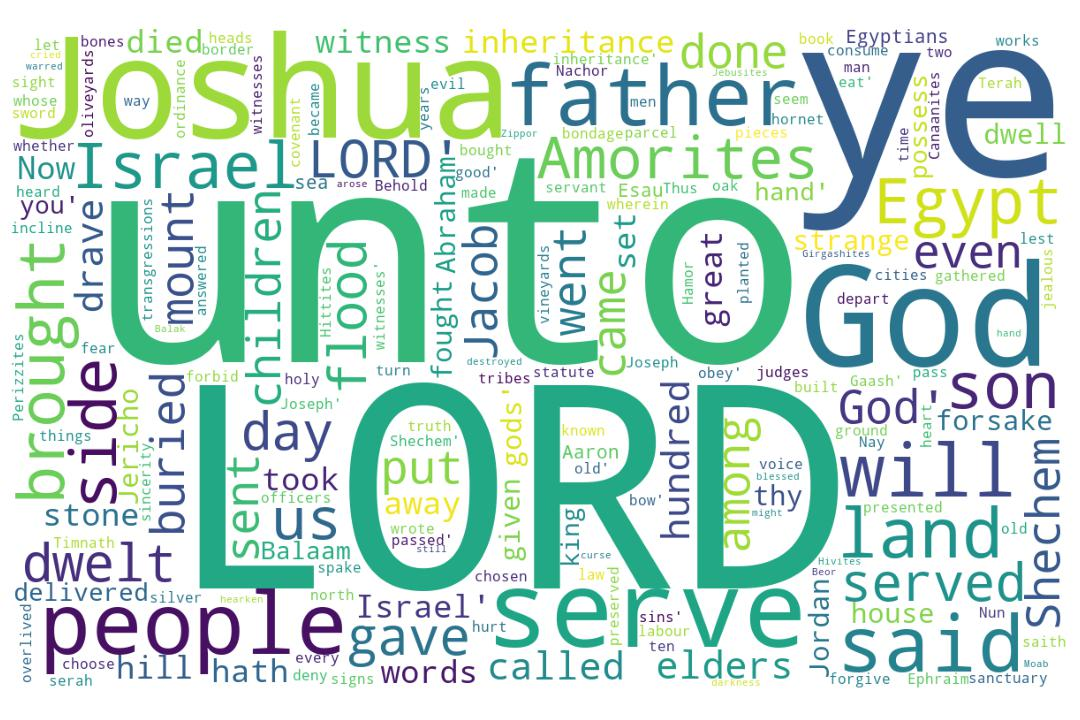
\includegraphics[width=\linewidth]{06OT-Joshua/Joshua24-WordCloud.jpg}
  \caption{Joshua 24 Word Cloud}
  \label{fig:Joshua 24 Word Cloud}
\end{figure}

\marginpar{\scriptsize \centering \fcolorbox{bone}{lime}{\textbf{JOSHUA'S SUMMARY}}\\ (Joshua 24)

\begin{compactenum}[I.][8]

	\item Story of a \textbf{Calling} \index[scripture]{Joshua!Jsh 24:03}(Jsh 24:3)
    \item Story of \textbf{Compassion} \index[scripture]{Joshua!Jsh 24:04}(Jsh 24:4)
    \item Story of \textbf{Covering} \index[scripture]{Joshua!Jsh 24:05}(Jsh 24:5)
    \item Story of \textbf{Conquering} \index[scripture]{Joshua!Jsh 24:08}(Jsh 24:8)
    \item Story of  \textbf{Commitment} \index[scripture]{Joshua!Jsh 24:14}(Jsh 24:14)
    \item Story of \textbf{Cleansing} \index[scripture]{Joshua!Jsh 24:23}(Jsh 24:23)
    \item Story of \textbf{Covenants} \index[scripture]{Joshua!Jsh 24:25}(Jsh 24:25)

\end{compactenum}}





\footnote{\textcolor[rgb]{0.00,0.25,0.00}{\hyperlink{TOC}{Return to end of Table of Contents.}}}\textcolor[cmyk]{0.99998,1,0,0}{And \fcolorbox{bone}{bone}{Joshua} gathered all the tribes of Israel to Shechem, and called for the elders of Israel, and for their heads, and for their judges, and for their officers; and they presented themselves before God.}
[2] \textcolor[cmyk]{0.99998,1,0,0}{And \fcolorbox{bone}{bone}{Joshua} said unto all the people, Thus saith the LORD God of Israel, Your fathers dwelt on the other side of the flood in old time, \emph{even} Terah, the father of Abraham, and the father of Nachor: and they served other gods.}
[3] \textcolor[cmyk]{0.99998,1,0,0}{And I took your father Abraham from the other side of the flood, and led him throughout all the land of Canaan, and multiplied his seed, and gave him Isaac.}\
[4] \textcolor[cmyk]{0.99998,1,0,0}{And I gave unto Isaac Jacob and Esau: and I gave unto Esau mount Seir, to possess it; but Jacob and his children went down into Egypt.}
[5] \textcolor[cmyk]{0.99998,1,0,0}{I sent Moses also and Aaron, and I plagued Egypt, according to that which I did among them: and afterward I brought you out.}
[6] \textcolor[cmyk]{0.99998,1,0,0}{And I brought your fathers out of Egypt: and ye came unto the sea; and the Egyptians pursued after your fathers with chariots and horsemen unto the Red sea.}
[7] \textcolor[cmyk]{0.99998,1,0,0}{And when they cried unto the LORD, he put darkness between you and the Egyptians, and brought the sea upon them, and covered them; and your eyes have seen what I have done in Egypt: and ye dwelt in the wilderness a long season.}
[8] \textcolor[cmyk]{0.99998,1,0,0}{And I brought you into the land of the Amorites, which dwelt on the other side Jordan; and they fought with you: and I gave them into your hand, that ye might possess their land; and I destroyed them from before you.}
[9] \textcolor[cmyk]{0.99998,1,0,0}{Then Balak the son of Zippor, king of Moab, arose and warred against Israel, and sent and called Balaam the son of Beor to curse you:}
[10] \textcolor[cmyk]{0.99998,1,0,0}{But I would not hearken unto Balaam; therefore he blessed you still: so I delivered you out of his hand.}
[11] \textcolor[cmyk]{0.99998,1,0,0}{And ye went over Jordan, and came unto Jericho: and the men of Jericho fought against you, the Amorites, and the Perizzites, and the Canaanites, and the Hittites, and the Girgashites, the Hivites, and the Jebusites; and I delivered them into your hand.}
[12] \textcolor[cmyk]{0.99998,1,0,0}{And I sent the hornet before you, which drave them out from before you, \emph{even} the two kings of the Amorites; \emph{but} not with thy sword, nor with thy bow.}
[13] \textcolor[cmyk]{0.99998,1,0,0}{And I have given you a land for which ye did not labour, and cities which ye built not, and ye dwell in them; of the vineyards and oliveyards which ye planted not do ye eat.}\\
\\
\P \textcolor[cmyk]{0.99998,1,0,0}{Now therefore fear the LORD, and serve him in sincerity and in truth: and put away the gods which your fathers served on the other side of the flood, and in Egypt; and serve ye the LORD.}
[15] \textcolor[cmyk]{0.99998,1,0,0}{And if it seem evil unto you to serve the LORD, choose you this day whom ye will serve; whether the gods which your fathers served that \emph{were} on the other side of the flood, or the gods of the Amorites, in whose land ye dwell: but as for me and my house, we will serve the LORD.}
[16] \textcolor[cmyk]{0.99998,1,0,0}{And the people answered and said, God forbid that we should forsake the LORD, to serve other gods;}
[17] \textcolor[cmyk]{0.99998,1,0,0}{For the LORD our God, he \emph{it} \emph{is} that brought us up and our fathers out of the land of Egypt, from the house of bondage, and which did those great signs in our sight, and preserved us in all the way wherein we went, and among all the people through whom we passed:}
[18] \textcolor[cmyk]{0.99998,1,0,0}{And the LORD drave out from before us all the people, even the Amorites which dwelt in the land: \emph{therefore} will we also serve the LORD; for he \emph{is} our God.}
[19] \textcolor[cmyk]{0.99998,1,0,0}{And \fcolorbox{bone}{bone}{Joshua} said unto the people, Ye cannot serve the LORD: for he \emph{is} an holy God; he \emph{is} a jealous God; he will not forgive your transgressions nor your sins.}
[20] \textcolor[cmyk]{0.99998,1,0,0}{If ye forsake the LORD, and serve strange gods, then he will turn and do you hurt, and consume you, after that he hath done you good.}
[21] \textcolor[cmyk]{0.99998,1,0,0}{And the people said unto \fcolorbox{bone}{bone}{Joshua}, Nay; but we will serve the LORD.}
[22] \textcolor[cmyk]{0.99998,1,0,0}{And \fcolorbox{bone}{bone}{Joshua} said unto the people, Ye \emph{are} witnesses against yourselves that ye have chosen you the LORD, to serve him. And they said, \emph{We} \emph{are} witnesses.}
[23] \textcolor[cmyk]{0.99998,1,0,0}{Now therefore put away, \emph{said} \emph{he}, the strange gods which \emph{are} among you, and incline your heart unto the LORD God of Israel.}
[24] \textcolor[cmyk]{0.99998,1,0,0}{And the people said unto \fcolorbox{bone}{bone}{Joshua}, The LORD our God will we serve, and his voice will we obey.}
[25] \textcolor[cmyk]{0.99998,1,0,0}{So \fcolorbox{bone}{bone}{Joshua} made a covenant with the people that day, and set them a statute and an ordinance in Shechem.}\\
\\
\P \textcolor[cmyk]{0.99998,1,0,0}{And \fcolorbox{bone}{bone}{Joshua} wrote these words in the book of the law of God, and took a great stone, and set it up there under an oak, that \emph{was} by the sanctuary of the LORD.}
[27] \textcolor[cmyk]{0.99998,1,0,0}{And \fcolorbox{bone}{bone}{Joshua} said unto all the people, Behold, this stone shall be a witness unto us; for it hath heard all the words of the LORD which he spake unto us: it shall be therefore a witness unto you, lest ye deny your God.}
[28] \textcolor[cmyk]{0.99998,1,0,0}{So \fcolorbox{bone}{bone}{Joshua} let the people depart, every man unto his inheritance.}\\
\\
\P \textcolor[cmyk]{0.99998,1,0,0}{And it came to pass after these things, that \fcolorbox{bone}{bone}{Joshua} the son of Nun, the servant of the LORD, died, \emph{being} an hundred and ten years old.}
[30] \textcolor[cmyk]{0.99998,1,0,0}{And they buried him in the border of his inheritance in Timnath-serah, which \emph{is} in mount Ephraim, on the north side of the hill of Gaash.}
[31] \textcolor[cmyk]{0.99998,1,0,0}{And Israel served the LORD all the days of \fcolorbox{bone}{bone}{Joshua}, and all the days of the elders that overlived \fcolorbox{bone}{bone}{Joshua}, and which had known all the works of the LORD, that he had done for Israel.}\\
\\
\P \textcolor[cmyk]{0.99998,1,0,0}{And the bones of Joseph, which the children of Israel brought up out of Egypt, buried they in Shechem, in a parcel of ground which Jacob bought of the sons of Hamor the father of Shechem for an hundred pieces of silver: and it became the inheritance of the children of Joseph.}
[33] \textcolor[cmyk]{0.99998,1,0,0}{And Eleazar the son of Aaron died; and they buried him in a hill \emph{that} \emph{pertained} \emph{to} Phinehas his son, which was given him in mount Ephraim.}



\chapter{Psalm 72}

\begin{figure}
  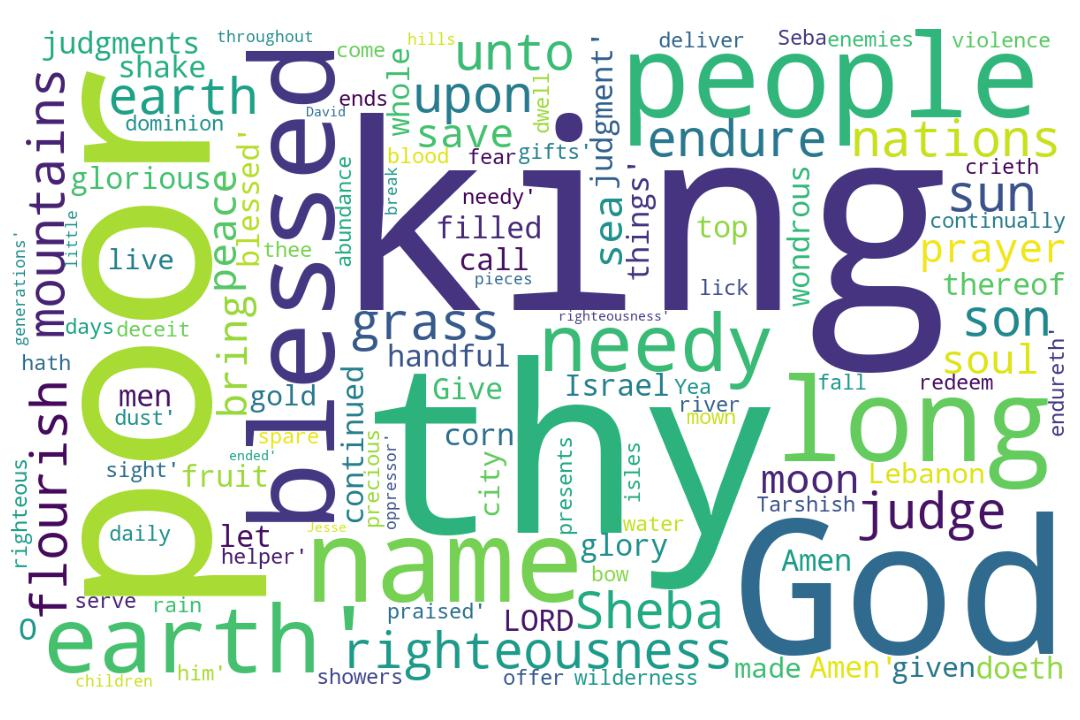
\includegraphics[width=\linewidth]{19OT-Psalms/Psalm72-WordCloud.jpg}
  \caption{Psalm 72 Word Cloud}
  \label{fig:Psalm 72 word Cloud}
\end{figure}


\marginpar{\scriptsize \centering \fcolorbox{bone}{lime}{\textbf{WITH THE PRINCE OF PEACE}}\\ (Psalm 72) \begin{compactenum}[I.][8]
    \item \textbf{Perfection in Judgment} \index[scripture]{Psalms!Psa 072:02}(Psa 72:2)
    \item The \textbf{Poor Blessed} \index[scripture]{Psalms!Psa 072:04}(Psa 72:4)
    \item \textbf{Peace Finally Arrives} \index[scripture]{Psalms!Psa 072:07}(Psa 72:7)
    \item \textbf{Opponents Praising} \index[scripture]{Psalms!Psa 072:09, 10}(Psa 72:9, 10)
    \item \textbf{Politics Centered on the Lord} \index[scripture]{Psalms!Psa 072:11}(Psa 72:11)
    \item \textbf{Produce Incredible} \index[scripture]{Psalms!Psa 072:16}(Psa 72:16)
    \item \textbf{Praise Continual} \index[scripture]{Psalms!Psa 072:17}(Psa 72:17)
\end{compactenum}}



\footnote{\textcolor[cmyk]{0.99998,1,0,0}{\hyperlink{TOC}{Return to end of Table of Contents.}}}\footnote{\href{https://audiobible.com/bible/psalms_72.html}{\textcolor[cmyk]{0.99998,1,0,0}{Psalm 72 Audio}}}\textcolor[cmyk]{0.99998,1,0,0}{\emph{A Psalm} for Solomon.}\\
\\
\textcolor[cmyk]{0.99998,1,0,0}{Give the king thy judgments, O God, and thy \fcolorbox{bone}{MYGOLD}{righteousness} unto the king's son.}
[2] \textcolor[cmyk]{0.99998,1,0,0}{He shall \fcolorbox{bone}{lime}{judge} thy people with \fcolorbox{bone}{MYGOLD}{righteousness}, and thy poor with judgment.}
[3] \textcolor[cmyk]{0.99998,1,0,0}{The mountains shall bring peace to the people, and the little hills, by \fcolorbox{bone}{MYGOLD}{righteousness}.}
[4] \textcolor[cmyk]{0.99998,1,0,0}{He shall judge the \fcolorbox{bone}{lime}{poor} of the people, he shall save the children of the needy, and shall break in pieces the oppressor.}
[5] \textcolor[cmyk]{0.99998,1,0,0}{They shall fear thee as long as the sun and moon endure, throughout all generations.}
[6] \textcolor[cmyk]{0.99998,1,0,0}{He shall come down like rain upon the mown grass: as showers \emph{that} water the earth.}
[7] \textcolor[cmyk]{0.99998,1,0,0}{In his days shall the righteous flourish; and abundance of \fcolorbox{bone}{lime}{peace} so long as the moon endureth.}
[8] \textcolor[cmyk]{0.99998,1,0,0}{He shall have dominion also from sea to sea, and from the river unto the ends of the earth.}\footnote{\textbf{Psalm 145:13} - Thy kingdom is an everlasting kingdom, and thy dominion endureth throughout all generations.}\footnote{\textbf{Zechariah 9:10} - And I will cut off the chariot from Ephraim, and the horse from Jerusalem, and the battle bow shall be cut off: and he shall speak peace unto the heathen: and his dominion shall be from sea even to sea, and from the river even to the ends of the earth.}\footnote{\textbf{Revelation 1:6} - And hath made us kings and priests unto God and his Father; to him be glory and dominion for ever and ever. Amen.}
[9] \textcolor[cmyk]{0.99998,1,0,0}{They that dwell in the wilderness shall \fcolorbox{bone}{lime}{bow before him}; and his enemies shall lick the dust.}
[10] \textcolor[cmyk]{0.99998,1,0,0}{The kings of Tarshish and of the isles shall bring presents: the kings of Sheba and Seba shall offer gifts.}
[11] \textcolor[cmyk]{0.99998,1,0,0}{Yea, all kings shall fall down \fcolorbox{bone}{lime}{before him}: all nations shall serve him.}
[12] \textcolor[cmyk]{0.99998,1,0,0}{For he shall deliver the needy when he crieth; the poor also, and \emph{him} that hath no helper.}
[13] \textcolor[cmyk]{0.99998,1,0,0}{He shall spare the poor and needy, and shall save the souls of the needy.}
[14] \textcolor[cmyk]{0.99998,1,0,0}{He shall redeem their soul from deceit and violence: and precious shall their blood be in his sight.}
[15] \textcolor[cmyk]{0.99998,1,0,0}{And he shall live, and to him shall be given of the gold of Sheba: prayer also shall be made for him continually; \emph{and} daily shall he be praised.}\footnote{\textbf{1 Kings 10:1-13} - And when the queen of Sheba heard of the fame of Solomon concerning the name of the LORD, she came to prove him with hard questions. [2] And she came to Jerusalem with a very great train, with camels that bare spices, and very much gold, and precious stones: and when she was come to Solomon, she communed with him of all that was in her heart. [3] And Solomon told her all her questions: there was not any thing hid from the king, which he told her not. [4] And when the queen of Sheba had seen all Solomon’s wisdom, and the house that he had built, [5] And the meat of his table, and the sitting of his servants, and the attendance of his ministers, and their apparel, and his cupbearers, and his ascent by which he went up unto the house of the LORD; there was no more spirit in her. [6] And she said to the king, It was a true report that I heard in mine own land of thy acts and of thy wisdom. [7] Howbeit I believed not the words, until I came, and mine eyes had seen it: and, behold, the half was not told me: thy wisdom and prosperity exceedeth the fame which I heard. [8] Happy are thy men, happy are these thy servants, which stand continually before thee, and that hear thy wisdom. [9] Blessed be the LORD thy God, which delighted in thee, to set thee on the throne of Israel: because the LORD loved Israel for ever, therefore made he thee king, to do judgment and justice. [10] And she gave the king an hundred and twenty talents of gold, and of spices very great store, and precious stones: there came no more such abundance of spices as these which the queen of Sheba gave to king Solomon. [11] And the navy also of Hiram, that brought gold from Ophir, brought in from Ophir great plenty of almug trees, and precious stones. [12] And the king made of the almug trees pillars for the house of the LORD, and for the king’s house, harps also and psalteries for singers: there came no such almug trees, nor were seen unto this day. [13] And king Solomon gave unto the queen of Sheba all her desire, whatsoever she asked, beside that which Solomon gave her of his royal bounty. So she turned and went to her own country, she and her servants.}\footnote{\textbf{Isaiah 60:6} - The multitude of camels shall cover thee, the dromedaries of Midian and Ephah; all they from Sheba shall come: they shall bring gold and incense; and they shall shew forth the praises of the LORD.}
[16] \textcolor[cmyk]{0.99998,1,0,0}{There shall be an handful of corn in the earth upon the top of the mountains; the \fcolorbox{bone}{lime}{fruit} thereof shall shake like Lebanon: and \emph{they} of the city shall flourish like grass of the earth.}
[17] \textcolor[cmyk]{0.99998,1,0,0}{His name shall endure for ever: his name shall be \fcolorbox{bone}{lime}{continued} as long as the sun: and \emph{men} shall be blessed in him: all nations shall call him blessed.}
[18] \textcolor[cmyk]{0.99998,1,0,0}{Blessed \emph{be} the LORD God, the God of Israel, who only doeth wondrous things.}
[19] \textcolor[cmyk]{0.99998,1,0,0}{And blessed \emph{be} his glorious name for ever: and let the whole earth be filled \emph{with} his glory; Amen, and Amen.}
[20] \textcolor[cmyk]{0.99998,1,0,0}{The prayers of David the son of Jesse are ended.}



\chapter{Proverb 13}

\begin{figure}
  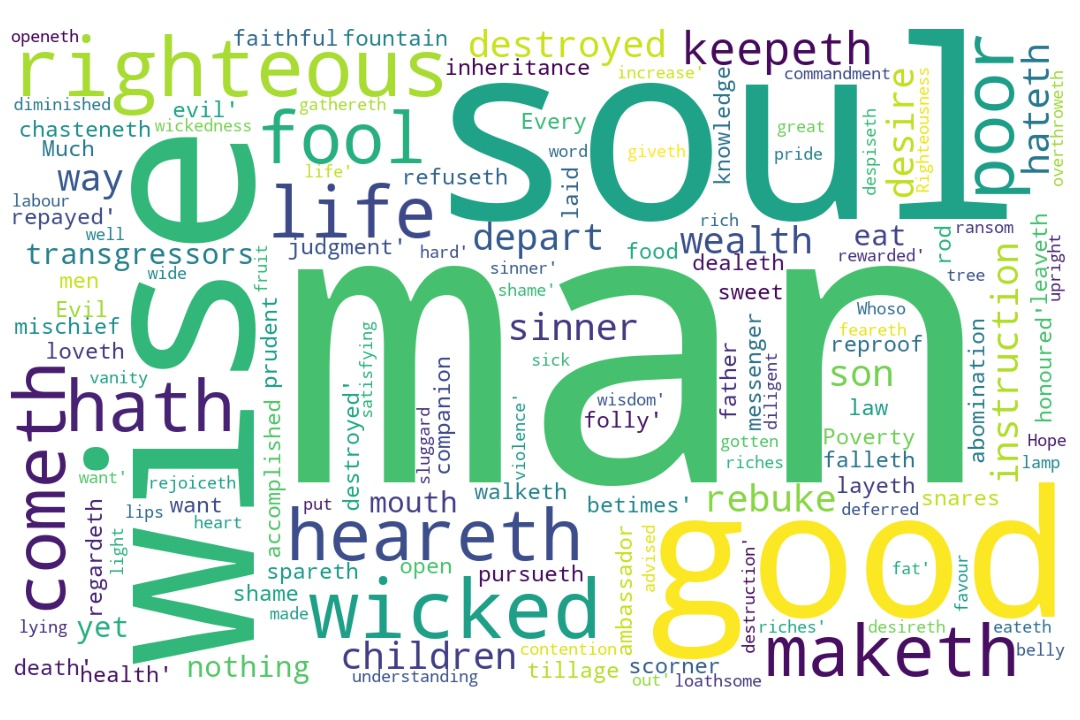
\includegraphics[width=\linewidth]{20OT-Proverbs/Proverb13-WordCloud.jpg}
  \caption{Proverb 13 Word Cloud}
  \label{fig:Proverb 13 Word Cloud}
\end{figure}

\marginpar{\scriptsize \centering \fcolorbox{bone}{lime}{\textbf{A WISE MAN}}\\ (Proverbs 13:1-25) \begin{compactenum}[I.][8]
    \item \textbf{Hears Instruction} \index[scripture]{Proverbs!Pro 13:01}(Pro 13:1)
    \item \textbf{Holds His Tongue} \index[scripture]{Proverbs!Pro 13:03}(Pro 13:3)
    \item \textbf{Hates Lying} \index[scripture]{Proverbs!Pro 13:05}(Pro 13:5)
    \item Is \textbf{Held up by Righteousness} \index[scripture]{Proverbs!Pro 13:06}(Pro 13:6)
    \item \textbf{Has True Wealth} \index[scripture]{Proverbs!Pro 13:07}(Pro 13:7)
    \item \textbf{Hearkens to God's Word} \index[scripture]{Proverbs!Pro 13:13}(Pro 13:13)
    \item \textbf{Hangs out with other wise Men} \index[scripture]{Proverbs!Pro 13:20}(Pro 13:20)
\end{compactenum}}

\marginpar{\scriptsize \centering \fcolorbox{bone}{yellow}{\textbf{A WISE SON}}\\ (Proverbs 13:1-25) \begin{compactenum}[I.][8]
    \item \textbf{Listens} to Instruction \index[scripture]{Proverbs!Pro 13:01}(Pro 13:1)
    \item \textbf{Learns}  \index[scripture]{Proverbs!Pro 13:01}(Pro 13:1)
    \item \textbf{Locks} his Lips \index[scripture]{Proverbs!Pro 13:03}(Pro 13:3)
    \item \textbf{Labours}  \index[scripture]{Proverbs!Pro 13:11}(Pro 13:11)
    \item \textbf{Likes} Reproof \index[scripture]{Proverbs!Pro 13:18}(Pro 13:18)
    \item \textbf{Leaves} an Inheritance \index[scripture]{Proverbs!Pro 13:22}(Pro 13:22)
    \item \textbf{Loves} Enough to Correct \index[scripture]{Proverbs!Pro 13:24}(Pro 13:24)
\end{compactenum}}

\footnote{\textcolor[cmyk]{0.99998,1,0,0}{\hyperlink{TOC}{Return to end of Table of Contents.}}}\footnote{\href{https://audiobible.com/bible/proverbs_13.html}{\textcolor[cmyk]{0.99998,1,0,0}{Proverbs Audio}}}\textcolor[cmyk]{0.99998,1,0,0}{A wise son \fcolorbox{bone}{lime}{\emph{heareth} his father's instruction}: but a scorner heareth not rebuke.}\footnote{\textbf{Isaiah 29:20} - For the terrible one is brought to nought, and the scorner is consumed, and all that watch for iniquity are cut off:}
[2] \textcolor[cmyk]{0.99998,1,0,0}{A man \fcolorbox{bone}{bone}{shall} eat good by the fruit of \emph{his} mouth: but the soul of the \fcolorbox{bone}{MYGOLD}{transgressors} \emph{\fcolorbox{bone}{bone}{shall}} \emph{eat} violence.}
[3] \textcolor[cmyk]{0.99998,1,0,0}{He that \fcolorbox{bone}{lime}{keepeth his mouth} keepeth his life: \emph{but} he that openeth wide his lips \fcolorbox{bone}{bone}{shall} have destruction.}
[4] \textcolor[cmyk]{0.99998,1,0,0}{The soul of the sluggard desireth, and \emph{hath} nothing: but the soul of the diligent \fcolorbox{bone}{bone}{shall} be made fat.}
[5] \textcolor[cmyk]{0.99998,1,0,0}{A righteous \emph{man} \fcolorbox{bone}{lime}{hateth lying}: but a wicked \emph{man} is loathsome, and cometh to shame.}
[6] \textcolor[cmyk]{0.99998,1,0,0}{\fcolorbox{bone}{MYGOLD}{Righteousness} keepeth \emph{him} \emph{that} \emph{is} upright in the way: but wickedness overthroweth the sinner.}
[7] \textcolor[cmyk]{0.99998,1,0,0}{There is that maketh himself rich, yet \emph{hath} nothing: \emph{there} \emph{is} that maketh himself poor, \fcolorbox{bone}{lime}{yet \emph{hath} great riches}.}
[8] \textcolor[cmyk]{0.99998,1,0,0}{The ransom of a man's life \emph{are} his riches: but the poor heareth not rebuke.}
[9] \textcolor[cmyk]{0.99998,1,0,0}{The light of the righteous rejoiceth: but the lamp of the wicked \fcolorbox{bone}{bone}{shall} be put out.}
[10] \textcolor[cmyk]{0.99998,1,0,0}{Only by pride cometh contention: but with the well advised \emph{is} wisdom.}
[11] \textcolor[cmyk]{0.99998,1,0,0}{Wealth \emph{gotten} by vanity \fcolorbox{bone}{bone}{shall} be diminished: but he that gathereth by labour \fcolorbox{bone}{bone}{shall} increase.}
[12] \textcolor[cmyk]{0.99998,1,0,0}{Hope deferred maketh the heart sick: but \emph{when} the desire cometh, \emph{it} \emph{is} a tree of life.}
[13] \textcolor[cmyk]{0.99998,1,0,0}{Whoso despiseth the word \fcolorbox{bone}{bone}{shall} be destroyed: but he that \fcolorbox{bone}{lime}{feareth the commandment} \fcolorbox{bone}{bone}{shall} be rewarded.}
[14] \textcolor[cmyk]{0.99998,1,0,0}{The law of the wise \emph{is} a fountain of life, to depart from the snares of death.}
[15] \textcolor[cmyk]{0.99998,1,0,0}{Good \fcolorbox{bone}{MYGOLD}{understanding} giveth favour: but the way of \fcolorbox{bone}{MYGOLD}{transgressors} \emph{is} hard.}
[16] \textcolor[cmyk]{0.99998,1,0,0}{Every prudent \emph{man} dealeth with knowledge: but a fool layeth open \emph{his} folly.}
[17] \textcolor[cmyk]{0.99998,1,0,0}{A wicked messenger falleth into mischief: but a faithful ambassador \emph{is} health.}
[18] \textcolor[cmyk]{0.99998,1,0,0}{Poverty and shame \emph{\fcolorbox{bone}{bone}{shall}} \emph{be} \emph{to} him that refuseth instruction: but he that regardeth reproof \fcolorbox{bone}{bone}{shall} be honoured.}
[19] \textcolor[cmyk]{0.99998,1,0,0}{The desire accomplished is sweet to the soul: but \emph{it} \emph{is} abomination to fools to depart from evil.}
[20] \textcolor[cmyk]{0.99998,1,0,0}{He that \fcolorbox{bone}{lime}{walketh with wise \emph{men}} \fcolorbox{bone}{bone}{shall} be wise: but a companion of fools \fcolorbox{bone}{bone}{shall} be destroyed.}\footnote{\textbf{2 Kings 9:11} - Then Jehu came forth to the servants of his lord: and one said unto him, Is all well? wherefore came this mad fellow to thee? And he said unto them, Ye know the man, and his communication.}\footnote{\textbf{1 Corinthians 15:33} - Be not deceived: evil communications corrupt good manners.}
[21] \textcolor[cmyk]{0.99998,1,0,0}{Evil pursueth sinners: but to the righteous good \fcolorbox{bone}{bone}{shall} be repayed.}
[22] \textcolor[cmyk]{0.99998,1,0,0}{A good \emph{man} leaveth an inheritance to his children's children: and the wealth of the sinner \emph{is} laid up for the just.}
[23] \textcolor[cmyk]{0.99998,1,0,0}{Much food \emph{is} \emph{in} the tillage of the poor: but there is \emph{that} \emph{is} destroyed for want of judgment.}
[24] \textcolor[cmyk]{0.99998,1,0,0}{He that spareth his rod hateth his son: but he that loveth him chasteneth him betimes.}
[25] \textcolor[cmyk]{0.99998,1,0,0}{The righteous eateth to the satisfying of his soul: but the belly of the wicked \fcolorbox{bone}{bone}{shall} want.}


% ransom , rebuke, refuseth, regardeth, rejoiceth, repayed, reproof, rewarded, rich, riches, righteous, rod


\end{document}

